\chapter{SSB in Redis}
% TODO: Kapitel linken
Der \emph{Star Schema Benchmark} wurde ursprünglich für relationale Datenbanken entwickelt, die auf SQL basieren. Er ist nicht ohne weiteres auf Key-Value-Stores wie \emph{Redis} übertragbar. In diesem Kapitel wird erläutert, wie die Daten und Abfragen des SSB angepasst werden können, um den Benchmark in Redis durchführen zu können.

In Kapitel ~\ref{sec:ssb-data-in-redis} werden Ansätze vorgestellt, wie die Daten innerhalb von Redis strukturiert werden können. Im Anschluss daran wird das im Rahmen dieser Arbeit entwickelte Programm \emph{SSB Inserter} zum Einfügen der Daten in Redis vorgestellt.


Kapitel ~\ref{sec:ssb-use-in-redis} beschäftigt sich mit der Ausführung des SSB in Redis.
Zunächst wird das entwickelte Programm \emph{Redis OLAP Client} vorgestellt, welches zur Ausführung der Queries verwendet wurde. Anschließend werden verschiedene Ansätze zur Durchführung der Queries erläutert.

\section{Herausforderungen}
%\subsection{Keine Joins}

% TODO: Irgendwo noch Test von SSB in PostgreSQL
\section{SSB Daten in Redis}\label{sec:ssb-data-in-redis}

% TODO: Hier ganze Anleitung im Anhang verlinken
\subsection{Generieren von SSB Daten}
Um Daten für einen \emph{Star Schema Benchmark} zu generieren, stellen die Autoren ein spezielles Tool~\cite{phillips_electrumssb-dbgen_2023} zur Verfügung.
Das in \emph{C} programmierte Tool ermöglicht nach der Kompilierung die Erstellung von \emph{.tbl}-Dateien, welche für den Import in SQL-basierte Datenbanksysteme geeignet sind.
Es erlaubt die Variation der Datenmenge durch Anpassung eines Parameters, um unterschiedliche Skalierungen zu generieren.
Das Tool basiert auf einem Programm, das ursprünglich zur Datengenerierung für den TPC-H-Benchmark entwickelt wurde.
\begin{lstlisting}[
    caption=Auszug aus generierter supplier.tbl-Datei,
    label=code:ssb-dbgen-example,
    numbers=none
]
92|Supplier#000000092|n48Wy4QI3lm|BRAZIL   7|BRAZIL|AMERICA|12-446-416-8471|
93|Supplier#000000093|wd1djjKXT|MOZAMBIQU9|MOZAMBIQUE|AFRICA|26-359-388-5266|
\end{lstlisting}
Die Zeilen der .tbl-Datei repräsentieren eine Zeile in einer Datenbanktabelle. Die einzelnen Spalten sind durch einen Trennstrich voneinander getrennt.
Beim Importieren der Daten werden die Spalten den entsprechenden Spalten in der Datenbank zugeordnet. Dafür muss die Tabelle im korrekten Format erstellt werden.

\subsection{Sternschema in Redis abbilden}
Bei der Betrachtung der Datenorganisation gibt es grundlegende Unterschiede zwischen dem \emph{Sternschema} und den Möglichkeiten zur Datenmodellierung in \emph{Redis}. Während das Sternschema trotz einer geringeren Normalisierung als einige andere Schemata mehrere Tabellen umfasst, fehlt das Konzept der Tabelle in \emph{Redis} vollständig.

\subsubsection{Modellierung der Daten mit künstlichen Namensräumen}
Um dennoch eine Art Tabellenstruktur in \emph{Redis} zu erreichen, werden durch das Hinzufügen von Präfixen zu Schlüsseln künstliche Namensräume geschaffen. Alle Einträge, die der Tabelle \emph{Supplier} angehören, beginnen beispielsweise mit dem Präfix \enquote{supplier:}. Durch dieses Vorgehen ist es möglich, bei der Nutzung von Befehlen wie \emph{Scan} oder bei der Anwendung von Indizes in \emph{RediSearch} gezielt nach diesem Präfix zu suchen. Die Methode wird dabei von \emph{RedisInsight} unterstützt, das die Möglichkeit bietet, Daten in der Benutzeroberfläche nach Präfixen gruppiert anzuzeigen.

Es besteht die Möglichkeit, mehrere \emph{Datenbanken} in Redis anzulegen.
Dies wird jedoch als Anti-Pattern angesehen und ist daher nicht empfohlen~\cite{prickett_answer_2022}. Viele Erweiterungen unterstützen nur die erste Datenbank. Daher wird der Ansatz der künstlichen Namensräume bevorzugt. 

Neben der Option, die Struktur der \emph{SSB}-Daten durch künstliche Namensräume darzustellen, besteht auch die Möglichkeit, die Daten vollständig zu denormalisieren. Kapitel \ref{sec:ssb-inserter} beschreibt die Umsetzung beider Ansätze.


\subsubsection{Wahl des Datentypen in Redis}
Von den gängigen Datentypen in Redis unterstützen nur Hashes, JSON und Sorted Sets eine Key-Value-Struktur. Theoretisch können Daten auch in Strings gespeichert werden und durch die Volltextsuche von Redisearch ist es auch möglich nach Daten zu suchen, jedoch ist dies wesentlich komplizierter als bei Hashes und JSON.
In Sorted Sets können nur begrenzte numerische Werte gespeichert werden was sie für die SSB-Daten nicht nutzbar macht, da dort unter anderem auch Texte gespeichert werden müssen.
Hashes und JSON bieten beide die Möglichkeit, beliebige Daten in einer Key-Value-Struktur zu speichern und dann mir RediSearch auch nach diesen Daten zu suchen.
Hashes benötigen dafür jedoch erheblich weniger Speicherplatz als JSON.
JSON wird in einer deserialisierten Form gespeichert und benötigt etwas Overhead zusätzlich zu den eigentlichen Daten~\cite{redis_ltd_json-ram-usage_nodate}.
Hashes sind dagegen optimiert um Speicher zu sparen~\cite{redis_ltd_memory-optimization_nodate}.
Mit dem Befehl \texttt{MEMORY USAGE} kann der Speicherverbrauch eines Elements in Redis angezeigt werden~\cite{redis_ltd_memory-usage-command-redis_nodate}.

% Dafür sorgen dass Abbildung an richitger Stelle ist...
In \Cref{pic:redis-hash-vs-json-memory} wird der Vergleich der Speicherplatznutzung dargestellt, wobei dieselben Informationen einmal in Form eines Hash und einmal in Form von JSON gespeichert sind. In diesem Beispiel belegt das JSON-Format 694 Byte, während das Hash-Format nur 288 Byte benötigt, was einer Reduzierung um 58,5\% entspricht.
\begin{figure}[!h]  % force the figure to be placed here
    \centering
    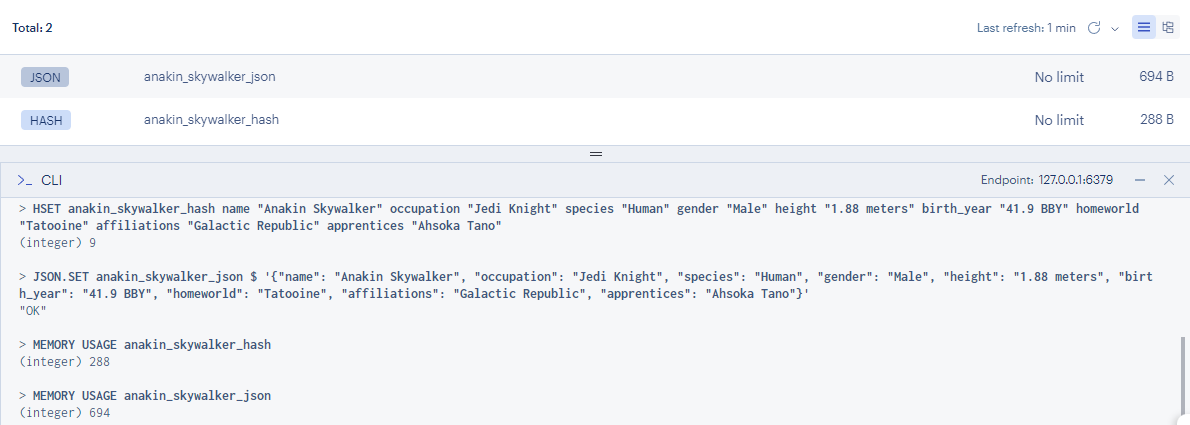
\includegraphics[width=1\textwidth]{pictures/redis/redis_hash_vs_json_memory.png}
    \caption{Vergleich des Speicherplatznutzung zwischen HASH und JSON}
    \label{pic:redis-hash-vs-json-memory}
\end{figure}

\subsection{SSB Inserter}\label{sec:ssb-inserter}

\subsubsection{Konfiguration von RediSearch und Jedis}
Redis verfügt über Eigenschaften, die beim Einfügen großer Datenmengen suboptimal sein können.
Es bietet die Möglichkeit, Daten sowohl als Snapshot als auch in einer Append-Only-Datei zu speichern (siehe Dokumentation von Redis~\cite{redis_ltd_persistence_nodate}).
Beim Einfügen von vielen Daten besteht die Gefahr, dass mehrfach Daten gespeichert werden, die in kurzer Zeit nicht mehr aktuell sind, wenn weitere Daten eingefügt werden. Aus diesem Grund wird beim Start des Programms sichergestellt, dass beide Optionen in der Konfiguration deaktiviert sind. Nachdem die Daten eingefügt wurden werden die Optionen wieder angepasst. 

Jedis hat außerdem einen Timeout für Anfragen. Um sicherzustellen, dass dieser Timeout das Einfügen der Daten nicht beendet, wird er auf unendlich gesetzt.

\begin{lstlisting}[
    caption=Optimierung beim Einfügen von Daten,
    label=code:ssb-inserter-redis-config,
    language=Scala
]
// before inserting
jedis.configSet("appendonly", "no")
jedis.configSet("save", "")
jedis.getClient.setTimeoutInfinite()

// after inserting
jedis.configSet("appendonly", "yes")
jedis.configSet("save", "3600 1")
// perform snapshot every hour if at least one key has been changed
\end{lstlisting}


\section{SSB in Redis ausführen}\label{sec:ssb-use-in-redis}

\subsection{Redis OLAP Client}

\subsubsection{Konfiguration von RediSearch und Jedis}
Standardmäßig begrenzt RediSearch sowohl die Anzahl der Suchergebnisse als auch die der Aggregationsergebnisse (siehe Dokumentation von RediSearch~\cite{redis_ltd_configuration_nodate}). Außerdem verfügt RediSearch über einen Timeout für Abfragen. Um sicherzustellen, dass diese Begrenzungen bei der Verarbeitung großer Datenmengen nicht wirksam werden, werden sie deaktiviert.

Gleiches gilt für den Timeout von Jedis auf der Clientseite.
\begin{lstlisting}[
    caption=Konfiguration von RediSearch,
    label=code:redis-olap-client-config,
    language=Scala
]
jedisPooled.sendCommand(SearchCommand.CONFIG, "SET", "MAXSEARCHRESULTS", "-1")
jedisPooled.sendCommand(SearchCommand.CONFIG, "SET", "MAXAGGREGATERESULTS", "-1")
jedisPooled.sendCommand(SearchCommand.CONFIG, "SET", "TIMEOUT", "0")

jedis.getClient.setTimeoutInfinite()
\end{lstlisting}

\section{4 Ansätze}

\subsection{Ansatz 1: Alles in Keys}
\subsubsection{Aufbau der Daten}
\subsubsection{Aufbau der Abfragen}
\subsubsection{Ergebnisse}
\subsubsection{Fazit}


\subsection{Ansatz 2: Clientseitige Joins}
\subsubsection{Aufbau der Daten}
\subsubsection{Aufbau der Abfragen}
\subsubsection{Ergebnisse}
\subsubsection{Fazit}


\subsection{Ansatz 3: Serverseitige Joins}
\subsubsection{Aufbau der Daten}
\subsubsection{Aufbau der Abfragen}
\subsubsection{Ergebnisse}
\subsubsection{Fazit}


\subsection{Ansatz 4: Denormalisiert}
\subsubsection{Aufbau der Daten}
\subsubsection{Aufbau der Abfragen}
\subsubsection{Ergebnisse}
\subsubsection{Fazit}